% allgem. Dokumentenformat
\documentclass[a4paper,12pt,headsepline]{scrartcl}
%Variablen welche innerhalb der gesamten Arbeit zur Verfügung stehen sollen
\newcommand{\titleDocument}{Bachelor- / Masterarbeit}
\newcommand{\subjectDocument}{im Studiengang <Studiengang>}

% weitere Pakete
% Grafiken aus PNG Dateien einbinden
\usepackage{graphicx}

% Deutsche Sonderzeichen benutzen 
\usepackage{ngerman}

% deutsche Silbentrennung
\usepackage[ngerman]{babel}

% Eurozeichen einbinden
\usepackage[right]{eurosym}

% Umlaute unter UTF8 nutzen
\usepackage[utf8]{inputenc}

% Zeichenencoding
\usepackage[T1]{fontenc}

\usepackage{lmodern}
\usepackage{fix-cm}

% floatende Bilder ermöglichen
%\usepackage{floatflt}

% mehrseitige Tabellen ermöglichen
\usepackage{longtable}

% Unterstützung für Schriftarten
%\newcommand{\changefont}[3]{ 
%\fontfamily{#1} \fontseries{#2} \fontshape{#3} \selectfont}

% Packet für Seitenrandabständex und Einstellung für Seitenränder
\usepackage{geometry}
\geometry{left=3.5cm, right=2cm, top=2.5cm, bottom=2cm}

% Paket für Boxen im Text
\usepackage{fancybox}

% bricht lange URLs "schoen" um
\usepackage[hyphens,obeyspaces,spaces]{url}

% Paket für Textfarben
\usepackage{color}

% Mathematische Symbole importieren
\usepackage{amssymb}

% auf jeder Seite eine Überschrift (alt, zentriert)
%\pagestyle{headings}

% erzeugt Inhaltsverzeichnis mit Querverweisen zu den Kapiteln (PDF Version)
\usepackage[bookmarksnumbered,pdftitle={\titleDocument},hyperfootnotes=false]{hyperref} 
%\hypersetup{colorlinks, citecolor=red, linkcolor=blue, urlcolor=black}
%\hypersetup{colorlinks, citecolor=black, linkcolor= black, urlcolor=black}

% neue Kopfzeilen mit fancypaket
\usepackage{fancyhdr} %Paket laden
\pagestyle{fancy} %eigener Seitenstil
\fancyhf{} %alle Kopf- und Fußzeilenfelder bereinigen
\fancyhead[L]{\nouppercase{\leftmark}} %Kopfzeile links
\fancyhead[C]{} %zentrierte Kopfzeile
\fancyhead[R]{\thepage} %Kopfzeile rechts
\renewcommand{\headrulewidth}{0.4pt} %obere Trennlinie
%\fancyfoot[C]{\thepage} %Seitennummer
%\renewcommand{\footrulewidth}{0.4pt} %untere Trennlinie

% für Tabellen
\usepackage{array}

% Runde Klammern für Zitate
%\usepackage[numbers,round]{natbib}

% Festlegung Art der Zitierung - Havardmethode: Abkuerzung Autor + Jahr
\bibliographystyle{alphadin}

% Schaltet den zusätzlichen Zwischenraum ab, den LaTeX normalerweise nach einem Satzzeichen einfügt.
\frenchspacing

% Paket für Zeilenabstand
\usepackage{setspace}

% für Bildbezeichner
\usepackage{capt-of}

% für Stichwortverzeichnis
\usepackage{makeidx}

% für Listings
\usepackage{listings}
\lstset{numbers=left, numberstyle=\tiny, numbersep=5pt, keywordstyle=\color{black}\bfseries, stringstyle=\ttfamily,showstringspaces=false,basicstyle=\footnotesize,captionpos=b}
\lstset{language=java}

% Indexerstellung
\makeindex

% Abkürzungsverzeichnis
\usepackage[german]{nomencl}
\let\abbrev\nomenclature

% Abkürzungsverzeichnis LiveTex Version
\renewcommand{\nomname}{Abkürzungsverzeichnis}
\setlength{\nomlabelwidth}{.25\hsize}
\renewcommand{\nomlabel}[1]{#1 \dotfill}
\setlength{\nomitemsep}{-\parsep}
\makenomenclature
%\makeglossary

% Abkürzungsverzeichnis TeTEX Version
% \usepackage[german]{nomencl}
% \makenomenclature
% %\makeglossary
% \renewcommand{\nomname}{Abkürzungsverzeichnis}
% \setlength{\nomlabelwidth}{.25\hsize}
% \renewcommand{\nomlabel}[1]{#1 \dotfill}
% \setlength{\nomitemsep}{-\parsep}

% Disable single lines at the start of a paragraph (Schusterjungen)
\clubpenalty = 10000
% Disable single lines at the end of a paragraph (Hurenkinder)
\widowpenalty = 10000
\displaywidowpenalty = 10000

\begin{document}
% hier werden die Trennvorschläge inkludiert
%hier müssen alle Wörter rein, welche Latex von sich auch nicht korrekt trennt bzw. bei denen man die genaue Trennung vorgeben möchte
\hyphenation{
Film-pro-du-zen-ten
Lux-em-burg
Soft-ware-bau-steins
zeit-in-ten-siv
}

%Schriftart Helvetica
%\changefont{phv}{m}{n}

% Leere Seite am Anfang
\newpage
\thispagestyle{empty} % erzeugt Seite ohne Kopf- / Fusszeile
\section*{ }

% Titelseite %
% das Papierformat zuerst
%\documentclass[a4paper, 11pt]{article}

% deutsche Silbentrennung
%\usepackage[ngerman]{babel}

% wegen deutschen Umlauten
%\usepackage[ansinew]{inputenc}

% hier beginnt das Dokument
%\begin{document}


\thispagestyle{empty}

%\begin{figure}[t]
% \includegraphics[width=0.6\textwidth]{abb/fh_koeln_logo}
%\end{figure}

\begin{figure}[t]
 \centering
 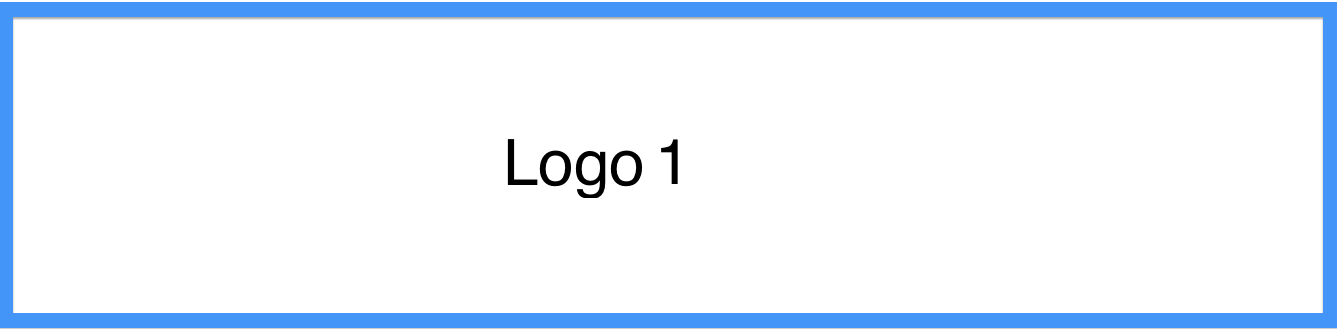
\includegraphics[width=0.6\textwidth]{abb/logo1}
~~~~~~~~~~
 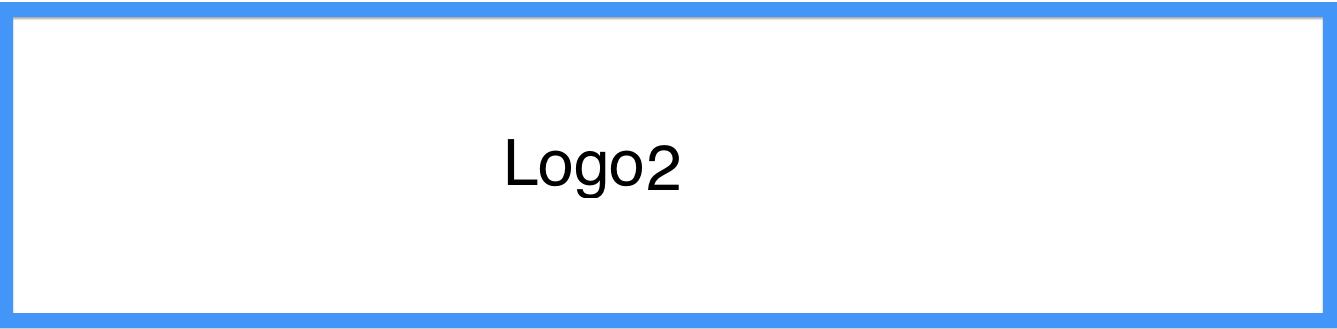
\includegraphics[width=0.3\textwidth]{abb/logo2}
\end{figure}


\begin{verbatim}


\end{verbatim}

\begin{center}
\Large{Fachhochschule <Name>}\\
\Large{- Campus <Name> -}\\
\end{center}


\begin{center}
\Large{Fakultät für <Fachrichtung>}
\end{center}
\begin{verbatim}




\end{verbatim}
\begin{center}
\doublespacing
\textbf{\LARGE{\titleDocument}}\\
\singlespacing
\begin{verbatim}

\end{verbatim}
\textbf{{~\subjectDocument~-~Schwerpunkt <Schwerpunktfach>}}
\end{center}
\begin{verbatim}

\end{verbatim}
\begin{center}

\end{center}
\begin{verbatim}

\end{verbatim}
\begin{center}
\textbf{zur Erlangung des akademischen Grades \\ Bachelor / Master of Science}
\end{center}
\begin{verbatim}






\end{verbatim}
\begin{flushleft}
\begin{tabular}{llll}
\textbf{Thema:} & & <Thema der Arbeit> & \\
& & \\
\textbf{Autor:} & & Name <name@mail.de>& \\
& & MatNr. 12345... & \\
& & \\
\textbf{Version vom:} & & \today &\\
& & \\
\textbf{1. Betreuerin:} & & Prof. Dr. X &\\
\textbf{2. Betreuer:} & & Prof. Dr. Y &\\
\end{tabular}
\end{flushleft}

% römische Numerierung
%\pagenumbering{arabic}

% 1.5 facher Zeilenabstand
\onehalfspacing

% Sperrvermerk
\section*{Sperrvermerk}
\textcolor{red}{
Die vorliegende Arbeit beinhaltet interne und vertrauliche Informationen der Firma <Firmenname>.
Die Weitergabe des Inhalts der Arbeit im Gesamten oder in Teilen sowie das Anfertigen
von Kopien oder Abschriften - auch in digitaler Form - sind grundsätzlich untersagt.
Ausnahmen bedürfen der schriftlichen Genehmigung der Firma <Firmenname>.
}

% Einleitung / Abstract
\section*{Zusammenfassung}


%\begin{verbatim}

%

%\end{verbatim}

\section*{Abstract}


% einfacher Zeilenabstand
\singlespacing

% Inhaltsverzeichnis anzeigen
\newpage
\tableofcontents

% das Abbildungsverzeichnis
%\newpage
% Abbildungsverzeichnis soll im Inhaltsverzeichnis auftauchen
\addcontentsline{toc}{section}{Abbildungsverzeichnis}
% Abbildungsverzeichnis endgueltig anzeigen
\listoffigures

% das Tabellenverzeichnis
%\newpage
% Abbildungsverzeichnis soll im Inhaltsverzeichnis auftauchen
\addcontentsline{toc}{section}{Tabellenverzeichnis}
% \fancyhead[L]{Abbildungsverzeichnis / Abkürzungsverzeichnis} %Kopfzeile links
% Abbildungsverzeichnis endgueltig anzeigen
\listoftables

%% WORKAROUND für Listings
%\makeatletter% --> De-TeX-FAQ
%\renewcommand*{\lstlistoflistings}{%
%  \begingroup
%    \if@twocolumn
%      \@restonecoltrue\onecolumn
%    \else
%      \@restonecolfalse
%    \fi
%    \lol@heading
%    \setlength{\parskip}{\z@}%
%    \setlength{\parindent}{\z@}%
%    \setlength{\parfillskip}{\z@ \@plus 1fil}%
%    \@starttoc{lol}%
%    \if@restonecol\twocolumn\fi
%  \endgroup
%}
%\makeatother% --> \makeatletter
% das Listingverzeichnis
%\newpage
% Listingverzeichnis soll im Inhaltsverzeichnis auftauchen
\addcontentsline{toc}{section}{Listingverzeichnis}
\fancyhead[L]{Abbildungs- / Tabellen- / Listingverzeichnis} %Kopfzeile links
\renewcommand{\lstlistlistingname}{Listingverzeichnis}
\lstlistoflistings
%%%%

% das Abkürzungsverzeichnis
%\newpage
% Abkürzungsverzeichnis soll im Inhaltsverzeichnis auftauchen
\addcontentsline{toc}{section}{Abkürzungsverzeichnis}
% das Abkürzungsverzeichnis entgültige Ausgeben
\fancyhead[L]{Abkürzungsverzeichnis} %Kopfzeile links
\nomenclature{UGC}{User Generated Content}
\nomenclature{CSS}{Cascading Style Sheets}
\nomenclature{JS}{JavaScript}
\nomenclature{SQL}{Structured Query Language}
\nomenclature{GPL}{GNU General Public License}
\nomenclature{GNU}{GNU is not Unix}
\nomenclature{LGPL}{GNU Lesser General Public License}
\nomenclature{XMPP}{Extensible Messaging and Presence Protocol}
\nomenclature{IM}{Instant Message}
\nomenclature{CMS}{Content Management System}
\nomenclature{RSS}{Really Simple Syndication}
\nomenclature{JSON}{JavaScript Object Notation}
\nomenclature{HTML}{Hypertext Markup Language}
\nomenclature{TDD}{Test-driven development}
\nomenclature{GUI}{Graphical User Interface}
\nomenclature{KPI}{Key Performance Indicator}
\nomenclature{WWW}{World Wide Web}
\nomenclature{OCR}{Optical Character Recognition}
\nomenclature{ERM}{Entity Relationship Modell}

\printnomenclature

% Definiert Stegbreite bei zweispaltigem Layout
\setlength{\columnsep}{25pt}

%%%%%%% EINLEITUNG %%%%%%%%%%%%
%\twocolumn
\newpage
\fancyhead[L]{\nouppercase{\leftmark}} %Kopfzeile links

% 1,5 facher Zeilenabstand
\onehalfspacing

% einzelne Kapitel
\section{Einleitung}\label{einleitung}


\section{Kapitel 1}\label{kapitel1}

\section{Kapitel 2}\label{kapitel2}

%....

\section{Ausblick}\label{ausblick}

\section{Fazit}\label{fazit}

% Beispiel für Bild mit Fußnote
\begin{figure}[htb]
 \centering
 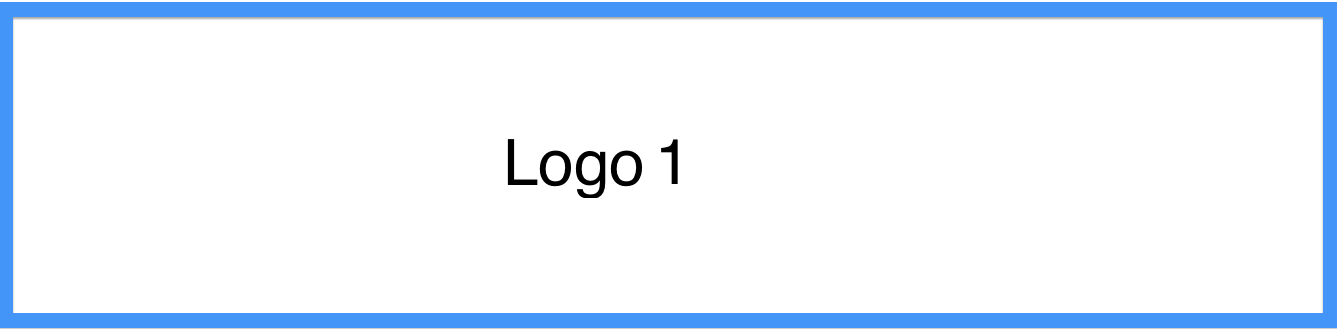
\includegraphics[width=0.4\textwidth,angle=45]{abb/logo1}
 \caption[Beispiel einer Bildbeschreibung]{Beispiel einer Bildbeschreibung\footnotemark}
\label{fig:beispiel1}
\end{figure}
\footnotetext{Bildquelle: Beispielquelle}

% Beispiel für Bildintegration
\begin{figure}[htb]
 \centering
 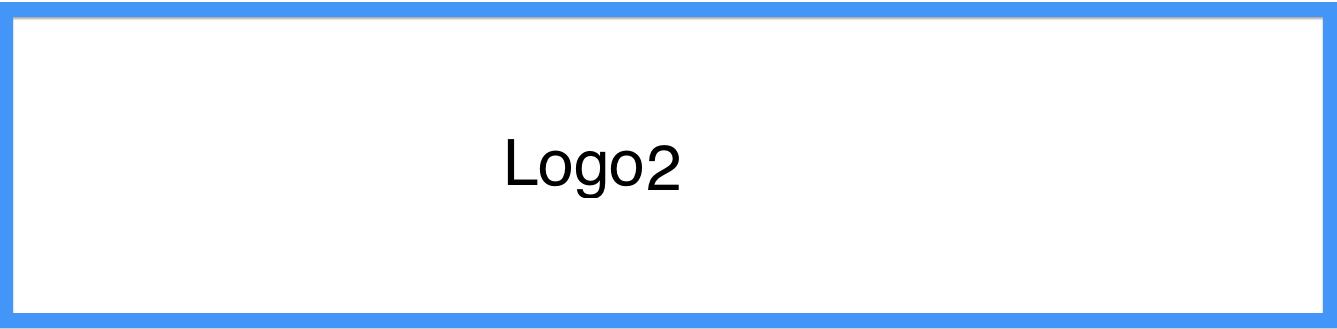
\includegraphics[width=0.3\textwidth,angle=0]{abb/logo2}
 \caption[Beschreibung]{Beschreibung}
\label{fig:Beschreibung}
\end{figure}

% Beispiel: Referenz auf Abbildung
Abbildung~\ref{fig:Beschreibung} [S.\pageref{fig:Beschreibung}]

% Beispiel: Tabelle 
\begin{center}
  \begin{tabular}{ | l | c | }
    \hline
    Überschrift 1 & Überschrift 2 \\ \hline \hline
    Info 1 & Info 2 \\ \hline
    Info 3 & Info 4 \\
    \hline
  \end{tabular}
\end{center}


% Beispiel für Quellcode Listings
\lstset{language=xml}
\begin{lstlisting}[frame=htrbl, caption={Die Datei {\tt data-config.xml} dient als Beispiel für XML Quellcode}, label={lst:dataconfigxml}]
<dataConfig>
  <dataSource type="JdbcDataSource" 
              driver="com.mysql.jdbc.Driver"
              url="jdbc:mysql://localhost/bms_db"
              user="root" 
              password=""/>
  <document>
    <entity name="id"
        query="select id, htmlBody, sentDate, sentFrom, subject, textBody
        from mail">
    <field column="id" name="id"/>
    <field column="htmlBody" name="text"/>
    <field column="sentDate" name="sentDate"/>
    <field column="sentFrom" name="sentFrom"/>
    <field column="subject"  name="subject"/>
    <field column="textBody" name="text"/>
    </entity>
  </document>
</dataConfig>
\end{lstlisting}

\lstset{language=java}
\begin{lstlisting}[frame=htrbl, caption={Das Listing zeigt Java Quellcode}, label={lst:result2}]
/* generate TagCloud */
Cloud cloud = new Cloud();
cloud.setMaxWeight(_maxSizeOfText);
cloud.setMinWeight(_minSizeOfText);
cloud.setTagCase(Case.LOWER);
	    
/* evaluate context and find additional stopwords */
String query = getContextQuery(_context);
List<String> contextStoplist = new ArrayList<String>();
contextStoplist = getStopwordsFromDB(query);
	    
/* append context stoplist */
while(contextStoplist != null && !contextStoplist.isEmpty())
  _stoplist.add(contextStoplist.remove(0));
	    
/* add cloud filters */
if (_stoplist != null) {
  DictionaryFilter df = new DictionaryFilter(_stoplist);
  cloud.addInputFilter(df);
}
/* remove empty tags */
NonNullFilter<Tag> nnf = new NonNullFilter<Tag>();
cloud.addInputFilter(nnf);

/* set minimum tag length */
MinLengthFilter mlf = new MinLengthFilter(_minTagLength);
cloud.addInputFilter(mlf);

/* add taglist to tagcloud */
cloud.addText(_taglist);

/* set number of shown tags */	    
cloud.setMaxTagsToDisplay(_tagsToDisplay);
\end{lstlisting}


% Beispiel für Formeln
Die Zuordnung aller möglichen Werte, welche eine Zufallsvariable annehmen kann nennt man \emph{Verteilungsfunktion} von $X$.

\begin{quotation}
Die Funktion F: $\mathbb{R} \rightarrow$ [0,1] mit $F(t) = P (X \le t)$ heißt Verteilungsfunktion von $X$.\footnote{Konen, vgl.~\cite{wk05}~[S.55]}
\end{quotation}

\begin{quotation}
Für eine stetige Zufallsvariable $X: \Omega \rightarrow \mathbb{R}$ heißt eine integrierbare, nichtnegative reelle Funktion $w: \mathbb{R} \rightarrow \mathbb{R}$ mit $F(x) = P(X \le x) = \int_{-\infty}^{x} w(t)dt$ die \emph{Dichte} oder \emph{Wahrscheinlichkeitsdichte} der Zufallsvariablen $X$.\footnote{Konen, vgl.~\cite{wk05}~[S.56]}
\end{quotation}


\onecolumn
% einfacher Zeilenabstand
\singlespacing
% Literaturliste soll im Inhaltsverzeichnis auftauchen
\newpage
\addcontentsline{toc}{section}{Literaturverzeichnis}
% Literaturverzeichnis anzeigen
\renewcommand\refname{Literaturverzeichnis}
\bibliography{Hauptdatei}

%% Index soll Stichwortverzeichnis heissen
% \newpage
% % Stichwortverzeichnis soll im Inhaltsverzeichnis auftauchen
% \addcontentsline{toc}{section}{Stichwortverzeichnis}
% \renewcommand{\indexname}{Stichwortverzeichnis}
% % Stichwortverzeichnis endgueltig anzeigen
% \printindex

\onehalfspacing
% evtl. Anhang
\newpage
\addcontentsline{toc}{section}{Anhang}
\fancyhead[L]{Anhang} %Kopfzeile links
\subsection*{Anhang}\label{anhang}


% Eidesstattliche Erklärung
\addcontentsline{toc}{section}{Eidesstattliche Erklärung}
\section*{Eidesstattliche Erklärung}
\thispagestyle{empty}

\begin{verbatim}

\end{verbatim}

\begin{LARGE}Eidesstattliche Erklärung zur <-Arbeit>\end{LARGE}
\begin{verbatim}


\end{verbatim}
Ich versichere, die von mir vorgelegte Arbeit selbstständig verfasst zu haben. Alle Stellen, die wörtlich oder sinngemäß aus veröffentlichten oder nicht veröffentlichten Arbeiten anderer entnommen sind, habe ich als entnommen kenntlich gemacht. Sämtliche Quellen und Hilfsmittel, die ich für die Arbeit benutzt habe, sind angegeben. Die Arbeit hat mit gleichem Inhalt bzw. in wesentlichen Teilen noch keiner anderen Prüfungsbehörde vorgelegen.



\begin{displaymath}
% use packages: array
\begin{array}{ll}
Unterschrift:~~~~~~~~~~~~~~~~~~~~~~~~~~~~~~~~~~~~~~~~~~
& Ort, Datum:~~~~~~~~~~~~~~~~~~~~~~~~~~~~~~~~~~~~~~~~~~
\end{array}
\end{displaymath}


% leere Abschlussseite
\newpage
\thispagestyle{empty} % erzeugt Seite ohne Kopf- / Fusszeile
\section*{ }

\end{document}